
\section{Auswertung}
\subsection{Bestimmung der Nullraten}
Durch die Nullrate kommt es schon bei Abwesenheit eines radioaktiven Strahlers zu einer geringen Zählrate.
Um die Messgenauigkeit zu verbessern, wird zuerst die Nullrate bestimmt. Diese
wird dann von den gemessenen Impulsen abgezogen.
\newline
Mit
\begin{equation}
  N_{0} = \frac{I_{0}}{t_{0}}
\end{equation}
ergeben sich die Nullraten für $\upgamma$- und $\upbeta$-Strahlung von
\begin{align*}
  N_{0,\upgamma} = \frac{651}{1000\,\su{s}} = (6,51\pm0,25) \cdot \num{e-1} \frac{1}{\su{s}}\\
  N_{0,\upbeta} = \frac{964}{1000\,\su{s}} = (9,64\pm0,31) \cdot \num{e-1} \frac{1}{\su{s}}.
\end{align*}
Die Fehler berechnen sich hierbei durch $N_{0} = \frac{\sqrt{I_{0}}}{t_{0}}$.
\subsection{Absorption von $\upgamma$-Strahlung}
Für die Messung der Absortption von $\upgamma$-Strahlung wird die Strahlungsquelle $^\text{137} \symup{Cs}$
verwendet. Die Absorptionskurven werden von den Materialien Blei Pb und Zink Zn aufegenommen.
\newline
Die aufgenommenen Messwerte sind aus Tabelle \ref{tab:blei} und \ref{tab:zink} zu entnehmen.
Die daraus resultierenden Graphen sind in Abbildungen \ref{fig:blei} und \ref{fig:zink} dargestellt.
\newline
Hierbei ist D die Dicke des jeweiligen Absorbers, t die gemessene Zeit und N die
Impulse. Die Aktivität berechnet sich aus $\Delta(N-N_{0})$. Der Fehler für die Aktivität
wird durch die Gauß Fehlerfortpflanzung
\begin{equation}
  \Delta(N-N_0)=\sqrt{(\symup{\Delta} N)^2+(\symup{\Delta} N_0)^2}
\end{equation}
bestimmt.
\newline
Aufgrund der Poissonverteilung ergeben sich die Fehler der gemessen Impulse durch
\begin{equation}
  \Delta(N) = \sqrt{N}.
\end{equation}
\begin{table}
\centering
\caption{Messwerte für die Absorptionskurve von Blei}
\label{tab:blei}
\begin{tabular}{S S S S}
\toprule
{$\su{D}\,/\,\text{mm}$} & {$\su{t}\,/\,\text{s}$} & {N} & {$\Delta(N-N_{0})$}\\
\midrule
1,2 & 50 & 6283\pm79 & 124,70\pm1,58 \\
2,4 & 60 & 7651\pm87 & 126,55\pm1,46 \\
12,0 & 80 & 4052\pm64 & 49,69\pm0,80 \\
13,2 & 90 & 4134\pm64 & 44,70\pm0,71 \\
24,0 & 120 & 2260\pm48 & 17,87\pm0,40 \\
25,2 & 140 & 2428\pm49 & 16,38\pm0,35 \\
34,5 & 180 & 1295\pm36 & 6,23\pm0,20 \\
35,7 & 210 & 1364\pm37 & 5,53\pm0,18 \\
44,0 & 300 & 873\pm30 & 1,95\pm0,1 \\
56,0 & 500 & 817\pm29 & 0,67\pm0,1 \\
\bottomrule
\end{tabular}
\end{table}
\begin{figure}
  \centering
  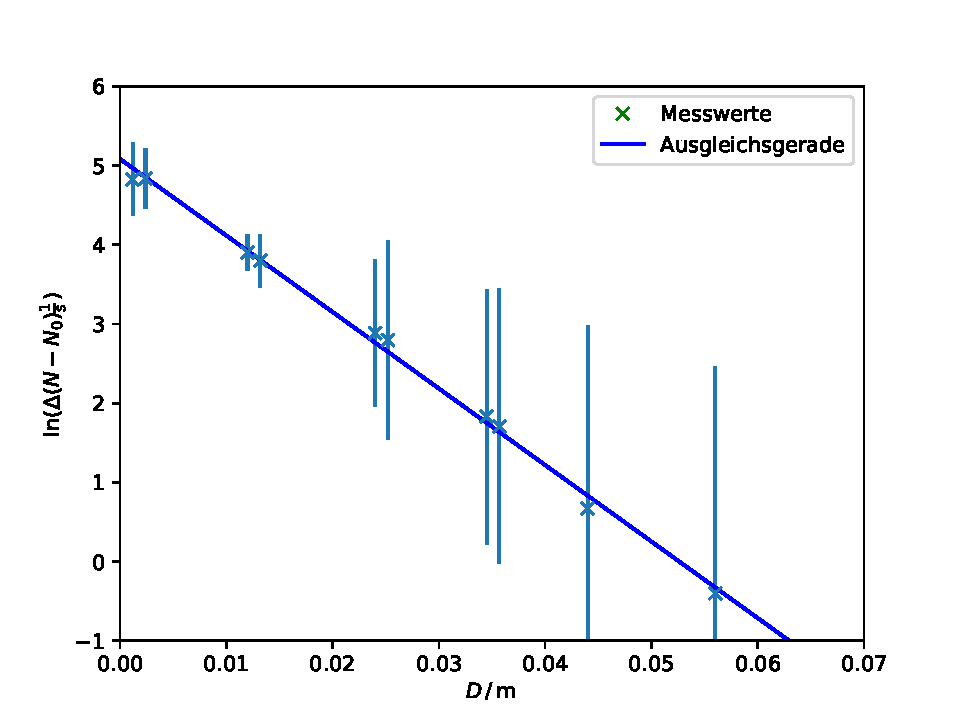
\includegraphics[scale=0.6]{blei.pdf}
  \caption{Absorptionskurve der $\upgamma$-Strahlung für Blei}
  \label{fig:blei}
\end{figure}
\begin{table}
\centering
\caption{Messwerte für die Absorptionskurve von Zink}
\label{tab:zink}
\begin{tabular}{S S S S}
\toprule
{$\su{D}\,/\,\text{mm}$} & {$\su{t}\,/\,\su{s}$} & {N} & {$\Delta\su{(N-N_{0})}$}\\
\midrule
2 & 30 & 4064\pm64 & 134,50\pm2,12 \\
4 & 40 & 5141\pm72 & 127,56\pm1,79 \\
6 & 50 & 6070\pm78 & 120,44\pm1,56 \\
8 & 60 & 6331\pm80 & 104,55\pm1,33 \\
10 & 65 & 6099\pm78 & 92,87\pm1,20 \\
12 & 70 & 6127\pm78 & 86,56\pm1,12 \\
14 & 80 & 6632\pm81 & 81,94\pm1,02 \\
16 & 90 & 6752\pm82 & 74,06\pm0,91 \\
18 & 100 & 6772\pm82 & 66,76\pm0,82 \\
20 & 110 & 7041\pm84 & 63,05\pm0,76 \\
\bottomrule
\end{tabular}
\end{table}
\begin{figure}
  \centering
  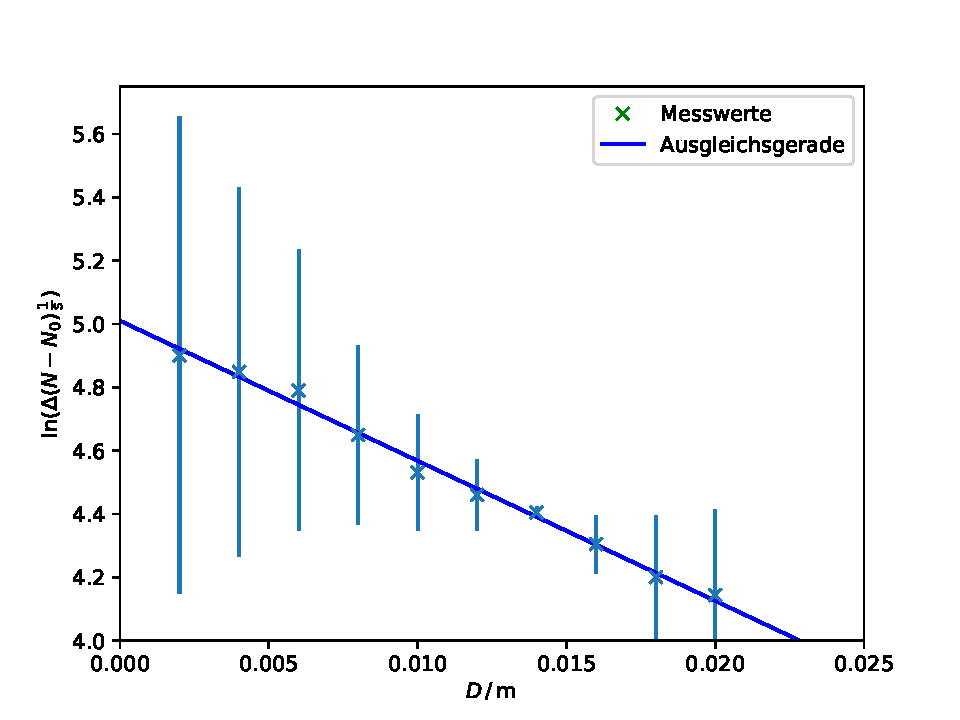
\includegraphics[scale=0.6]{zink.pdf}
  \caption{Absorptionskurve der $\upgamma$-Strahlung für Zink}
  \label{fig:zink}
\end{figure}
\newpage
Für beide Geraden wird eine Ausgleichsrechnung der Form
\begin{equation}
    \ln(\Delta (N-N_0))=\mu d + N_0
\end{equation}
durchgeführt.
\newline
Aus dieser Geradengleichung kann der Absorptionskoeffizient und die Anfangsaktivität $\su{N_0}$
bestimmmt werden. Diese Parameter sind in Tabelle \ref{tab:para} für Blei und Zink dargstellt.
\begin{table}
  \caption{Berechnete Parameter für die Absorptionskurven von Blei und Zink.}
  \label{tab:para}
  \centering
  \begin{tabular} {S S S}
    \toprule
     {Probe}& {$\mu_{\su{com,exp}}\,/\,\su{\frac{1}{m}}$} & {$N_0\,/\,\su{\frac{1}{s}}$}\\
    \midrule
      $\text{Blei}$ & 96,6\pm2 & 5,08\pm0,06\\
      $\text{Zink}$ & 44,2\pm1,4 & 5,01\pm0,02\\
    \end{tabular}
  \end{table}
\newline
Zur Bestimmung des theoretischen Absorptionskoeffizient $\mu_{\su{com}}$ wird zuerst der Wirkungsquerschnitt
$\sigma_{\su{com}}$ mit Formel \ref{eqn:sigma} bestimmt. Dafür wird $\epsilon = 1,295$ gesetzt. Die dafür benötigten Größen \cite{Lit1} sind in der folgenden Tabelle
zu finden. Der Absorptionskoeffizient wird dann über Formel \ref{eqn:absorption} berechnet.
  \begin{table}
    \caption{Wirkung von Blei und Zink.}
    \label{tab:wirkung}
    \centering
    \begin{tabular} {S S S S S S }
      \toprule
       {Probe}& {$\rho$\,/\,$\su{\frac{g}{cm^3}}$} & {M\,/\,$\su{\frac{g}{mol}}$} & {Z} & {$\sigma_{\text{com}}$\,/\,\num{e-25}$\su{cm^2}$}
       & {$\mu_{\text{com,theo}}$\,/\,$\su{\frac{1}{m}}$}\\
      \midrule
        $\text{Blei}$  & 11,34 & 207,2 & 82 & 2,57 & 69,458\\
        $\text{Zink}$  & 7,14  & 65,38 & 30 & 2,57 & 50,701\\
      \end{tabular}
    \end{table}
\newpage
\subsection{Absorption von $\upbeta$-Strahlung}
Für die Bestimmung der Absorptionskurve des $\upbeta$-Strahlers $^\text{99} \symup{Tc}$
wird Aluminium als Probe verwendet. Mithilfe der Absorptionskurve von Aluminium
wird dann die maximale Energie des Strahlers bestimmt.
\newline
Die Messwerte sind aus Tabelle \ref{tab:beta} zu entnehmen.
\begin{table}
\centering
\caption{Messwerte für die Absorptionskurve von Aluminium}
\label{tab:beta}
\begin{tabular}{S S S S}
\toprule
{$\su{D}\,/\,\su{\mu m}$} & {$\su{t}\,/\,\su{s}$} & {N} & {$\Delta(N-N_{0})$}\\
\midrule
100 & 60 & 2453\pm50 & 40,23\pm0,83 \\
125 & 60 & 608\pm25 & 9,48\pm0,41 \\
153 & 60 & 661\pm26 & 10,37\pm0,43\\
160 & 60 & 369\pm19 & 5,50\pm0,32 \\
200 & 80 & 168\pm13 & 1,45\pm0,16 \\
253 & 120 & 94\pm10 & 0,13\pm0,08\\
302 & 250 & 171\pm13 & 0,03\pm0,05 \\
338 & 450 & 307\pm18 & 0,03\pm0,03 \\
400 & 700 & 504\pm22 & 0,07\pm0,03 \\
444 & 900 & 645\pm25 & 0,07\pm0,02 \\
\bottomrule
\end{tabular}
\end{table}
\newline
Der aus den Messwerte folgende Graph ist in Abbildung \ref{fig:beta} dargestellt.
\begin{figure}
  \centering
  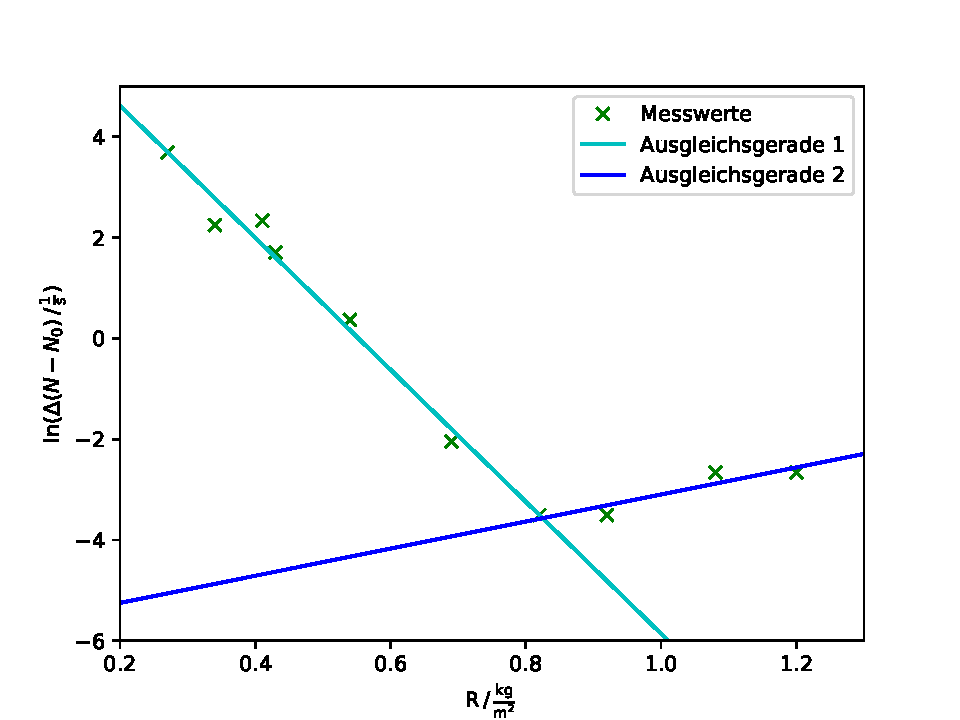
\includegraphics[scale=0.6]{beta.pdf}
  \caption{Absorptionskurve der $\upbeta$-Strahlung}
  \label{fig:beta}
\end{figure}
\newline
Die beiden linearen Ausgleichsgeraden der Form $y= Ax+B$ ergeben die Parameter
\begin{align*}
  A_{1} &= (-13,10\pm0,78)\,\su{\frac{1}{m}}\\
  B_{1} &= (7,24\pm0,79)\\
  A_{2} &= (2,69\pm0,78)\,\su{\frac{1}{m}}\\
  B_{2} &= (-5,78\pm0,79)\\
\end{align*}
Aus dem Schnittpunkt der Ausgleichsgeraden wird die maximale Reichweite der
$\upbeta$-Teilchen $R_{\su{max}}$ berechnet. Es ergibt sich ein Wert von
\begin{align*}
  R_{\su{max}} &= \frac{B_2 - B_1}{A_1 - A_2} = (0,82\pm0,09)\,\su{m}
\end{align*}
\newline
Die Maximalenergie des $^\text{99} \symup{Tc}$-Strahlers, die sich mit Formel \ref{eqn:E} berechnen lässt,
beträgt
\begin{align*}
  E_{\su{max}} &= (0,302\pm0,021)\,\su{MeV}.
\end{align*}
\section{Diskussion}
In der folgenden Tabelle sind die berechneten Werte für den Compton-Absorptionskoeffizienten nochmal
zusammengefasst.
\begin{table}
  \caption{$\upgamma$-Absorptionskoeffizienten im Vergleich}
  \label{tab:wirkung}
  \centering
  \begin{tabular} {S S S S}
    \toprule
     {Probe} & {$\mu_{\text{com,exp}}$\,/\,$\su{\frac{1}{m}}$} & {$\mu_{\text{com,theo}}$\,/\,$\su{\frac{1}{m}}$} & {Prozentuale Abweichung} \\
    \midrule
      $\text{Blei}$  & 96,6 & 69,458 & 39,07\,\% \\
      $\text{Zink}$  & 44,2 & 50,701 & 12,82\,\% \\
    \bottomrule
    \end{tabular}
  \end{table}
\newline
Für den Compton-Absorptionskoeffizienten von Blei folgt eine prozentuale Abweichung von
39$\%$ vom Theoriewert. Diese große Abweichung ist dadurch zu erklären, dass der Comptoneffekt
nicht alleine wirkt, sondern in dem Bereich auch der Photoeffekt berücksichtigt werden muss.
Im Vergleich zum Absorptionskoeffizient von Blei, ist die prozentuale Abweichung von Zink deutlich kleiner.
Sie beträgt 12$\%$. Zwar liegt diese nicht mehr im Toleranzbereich, jedoch scheinen bei Zink die
Wirkung vom Photoeffekt deutlich geringer zu sein. Trotzdem kann auch in diesem Fall nicht nur vom
Comptoneffekt ausgegangen werden.
\newline
Nicht nur die Berücksichtigung eines anderen Absorptionsmechanismus führt zu den prozentualen
Abweichung, sondern auch der Versuchsaufbau. Vorallem die Bleiplatten konnten nicht immer
exakt parallel zur $\upgamma$-Quelle eingebaut werden, da diese leicht verformbar sind.
\newline
Die Abweichung der maximalen Energie des $\upbeta$-Strahlers im Vergleich zu dem Literaturwert von
0,293\,MeV\cite{Lit2} beträgt nur 3\%. Im Graphen wird deutlich, dass nahe der maximalen Reichweite
starke Abweichungen vom Absorptionsgesetz durch Bremsstrahlung auftreten.
